%----------------------------------------
% SECTION:
%----------------------------------------
\section{Generalization to \texorpdfstring{$\Z_N$}{Z\_N}}%
\label{sec:generalization_to_zn}
In this section we are going to generalize the $\Z_2$ \ac{lgt} to a class of Abelian \ac{lgt} with discrete symmetry $\Z_N$.
This class is of particular interest because they approximate a $U(1)$ gauge theory in the limit $N to \infty$.



%
% SUBSECTION: Schwinger-Weyl algebra
%
\subsection{Schwinger-Weyl algebra}%
\label{sub:schwinger_weyl_algebra}

According to Wilson's Hamiltonian approach to \ac{lgt}s \cite{wilson1974confinement}, $U(1)$ gauge fields are defined on the links of a lattice $\Lattice$ either in a pair of conjugate variables, the electric field  $E_\link$ and either the vector potential $A_\link$, satisfying
\begin{equation}
    \comm{E_\link}{A_{\link^{\prime}}}  = i \delta_{\link , \link^{\prime} },
\end{equation}
or equivalently the \emph{magnetic operator}, also called \emph{comparator},
$U_\link = e^{-i A_{\link} }$, such that
\begin{equation}
    \comm{E_\link}{U_{\link^{\prime}}} =  \delta_{\link , \link^{\prime} } \, U_{\link},
\end{equation}
all acting on an infinite dimensional Hilbert space defined on each link $\link \in \Lattice$.
This form of the canonical commutation relations represents the infinitesimal version of the relations:
\begin{equation}
     e^{i\xi E} e^{-i\eta A } e^{-i\xi E} = e^{i\xi \eta} e^ {-i\eta A },
\end{equation}
for any $\xi, \eta \in \mathbb{R}$,
that define the Schwinger-Weyl group \cite{notarnicola2015discrete, ercolessi2018znmodels, schwinger1960unitary}.

For a discrete group like $\Z_N$, the notion of infinitesimal generators loses any meaning and we are led to directly consider, for each link $\link \in \Lattice$, two unitary operators
$V_\link, \, U_\link$, such that \cite{schwinger1960unitary, schwinger2001symbolism}
\begin{equation}
    V_\link U_\link V_\link^{\dagger}=e^{2\pi i/N}U_\link, \qquad
    U_\link^N=\identity_N, \qquad
    V_\link^N=\identity_N.
    \label{eq:schwinger_weyl_algebra}
\end{equation}
while they commute on different links.
Thus, by representing $\Z_N$  with the set of the $N$ roots of unity $e^{i 2 \pi k/N}$\, ($k=1, \cdots, N$), commonly referred to as the discretized circle,
we see that $V$ plays the role of a ``position operator'' on the discretized circle, while $U$ that of a ``momentum operator''.


\begin{figure}[t]
    \SideFigure[label=eq:link_operator_ZN, desc={Link operators in the $\Z_5$ case}]{%
        \begin{tikzpicture}[scale=1.1]
    \draw (1,0) arc (0:360:1);
    \foreach \angle in {72, 144, ..., 360}
    \node[site, fill=Yellow, minimum size=7pt] (state \angle) at (\angle:1) {};
    \draw (state 360.east) node[right] {$1$};
    \draw (state 72.north)  node[above] {$\omega$};
    \draw (state 144.west) node[above left] {$\omega^2$};
    \draw (state 216.west) node[left] {$\omega^{3}$};
    \draw (state 288.south) node[below] {$\omega^{4}$};

    \draw[Z, -stealth, shorten >=5pt] (0,0) -- (72:1) node [pos=0.5, left, black] {$V$};

    \draw[X, -stealth] (1.5, 0) arc (0:40:1.5) node [pos=0.5, right, black] {$U$};

    \draw (0,0) node[site, fill=black, draw=black] {};

\end{tikzpicture}

    }{%
        The operators $U$ and $V$ of a single link, in the $\Z_5$ case. The $V$ plays the role of a position operator, while $U$ that of a shift operator.
    }
\end{figure}


These algebraic relations admit a faithful finite-dimensional representation of dimension $N$ \cite{weyl1950theory}, for any integer $N$, which is obtained as follows.
To each link $\link$, we can associate an $N$-dimensional Hilbert space $\HilbertSpace_\link \simeq \C^N$.
As an orthonormal basis for $\HilbertSpace_\link$ we choose the \emph{electric basis} $\{\ket{v_{k,\link}}, k=1, \dots, N\}$, that diagonalizes the operator $V_\link$.
With this choice, we can promptly write the actions of $U_\link$ and $V_\link$:
\begin{equation}
    \begin{split}
        U_\link \ket{v_{k,\link}} & = \ket{v_{k+1,\link}}, \qquad \text{(mod $N$)} \\
        % U\ket{v_{N,\link}} = \ket{v_{1,\link}}\\
        V_\link \ket{v_{k,\link}} & = \omega^k \ket{v_{k,\link}},
    \end{split}
    \label{eq:elect_basis_op_action}
\end{equation}
where $\omega = e^{2 \pi i / N}$ and $k = 0, \dots, N-1$.
It is immediate to find the action for the Hermitian conjugates $U^{\dagger}_\link$ and $V^{\dagger}_\link$:
\begin{equation}
    \begin{split}
        U^\dagger_\link \ket{v_{k,\link}} & = \ket{v_{k-1,\link}}, \qquad \text{(mod $N$)} \\
        V^\dagger_\link \ket{v_{k,\link}} & = \omega^{-k} \ket{v_{k,\link}}.
    \end{split}
    \label{eq:elect_basis_op_action_hc}
\end{equation}
With this choice, $U_\link$ and $V_\link$ in matrix form are written as
\begin{equation}
    U_\link =
    \setlength\arraycolsep{5pt}
    \begin{pmatrix}
        0      & 0      & \cdots & \cdots & 1      \\
        1      & 0      & \cdots & \cdots & 0      \\[-5pt]
        0      & 1      & \ddots &        & . \\[-5pt]
        \vdots & \vdots & \ddots & \ddots & \vdots \\
        0      & 0      & \cdots & 1      & 0
    \end{pmatrix}
    \qand
    \setlength\arraycolsep{2pt}
    V_\link =
    \begin{pmatrix}
        1 \\
        & \omega \\
        &         & \omega^2 \\[-7pt]
        &         &           & \ddots \\[-2pt]
        &         &           &         & \omega^{N-1}
    \end{pmatrix}.
\end{equation}
We choose to work in this particular basis and the various $k$ can be interpreted as the quantized values of the electric field on the links.

In the $\Z_N$ case it is important to fix the orientation of the lattice $\Lattice$, because for $N \geq 3$ we have $U^{\dagger} \neq U$ and $V^{\dagger} \neq V$.
We choose the orientation shown in Fig.~\ref{fig:link_labels}.
On a two-dimensional square lattice of size $L \times L$, the links $\link$ of the lattice can also be labeled with $(x, \pm\hat{i})$, where $x \in \Lattice$ is a site and
$\hat{i}=\hat{1}, \hat{2}$ the two independent unit vectors.
In this way, $(x, \pm\hat{i})$ will refer to the link that start in $x$ and goes in the positive (negative) direction~$\hat{i}$.
As we will see later, the choice of the orientation affects the definition of any string operator.
The general rule for when defining a string operator as a product of $\mathcal{O}$ operators, where $\mathcal{O}$ is either $U$ or $V$ for example, is to use $\mathcal{O}$ when going in the positive direction or $\mathcal{O}^{\dagger}$ otherwise.
%This notation will be simplified when we reduce to the ladder case.


\begin{figure}
    \SideFigure[label=fig:link_labels, desc={Sites and links in a two-dimensional lattice}]{%
        \begin{tikzpicture}[
        font=\footnotesize,
        scale=1.3,
        site/.style = {circle, inner sep=0 pt, minimum size=5pt, draw=black, fill=white},
        decoration={
            markings,
            mark=at position 0.35 with {\arrow{>}},
            mark=at position 0.85 with {\arrow{>}}
        }
    ]
    % Lattice
    \draw[Gray, thin] (-1.75, -1.5) grid (1.75, 1.5);
    % links
    \draw[very thick, postaction={decorate}]
        (-1, 0) -- (1, 0)
        node [pos=0.75, below] {$(x, \hat{1})$}
        % node [pos=0.25, below] {$(x, -\hat{1})$}
        ;
    \draw[very thick, postaction={decorate}]
        (0, -1) -- (0, 1)
        node [pos=0.8, right] {$(x, \hat{2})$}
        % node [pos=0.15, right] {$(x, -\hat{2})$}
        ;
    % sites
    \foreach \x in {-1,...,1}
        \foreach \y in {-1,...,1}
            \draw (\x, \y) node [site] {};
    \draw (0, 0) node [Gray, above right] {$x$};
    \draw (1, 0) node [Gray, above right] {$x + \hat{1}$};
    \draw (0, 1) node [Gray, above right] {$x + \hat{2}$};
\end{tikzpicture}

    }{%
        Labelling of the sites and the links in the two dimensional lattice.
        A site is labeled simply with $x = (x_1, x_2)$, while $\hat{1} = (1,0)$ and $\hat{2} = (0,1)$ stand for the unit vectors of the lattice.
        A link $\link$ is denoted with a pair $(x, \pm\hat{i})$, with $\hat{i} = \hat{1}, \hat{2}$.
    }
\end{figure}


%
% SUBSECTION: Schwinger-Weyl algebra
%
\subsection{Gauge invariance and Hamiltonian}%
\label{sub:gauge_invariance_and_hamiltonian}

Gauge transformations transforms the vector potential while preserving the electric field.
For a $U(1)$ gauge theory, a local phase transformation is induced by a real function $\alpha_x$
defined on the vertices $x\in \mathbb L$, such that  $A_{\link} \mapsto A_{\link} + (\alpha_{x_2} - \alpha_{x_1})$ or equivalently
\begin{equation}
    U_{\link} \mapsto
    e^{i(\alpha_{x_2} - \alpha_{x_1}) E_{\link}}  U_{\link}   e^{-i(\alpha_{x_2} - \alpha_{x_1} )E_{\link}},
\end{equation}
where $x_1, x_2$ are the initial and final vertices of the (directed) link $\link$.
In the case of a discrete symmetry, a gauge transformation at a site $x \in \Lattice$ is a product of $V$'s (and $V^\dagger$'s) defined on the links which comes out (and enters) the vertex.
More specifically, for a two dimensional lattice,
if the link $\link$ at site $x$ is oriented in the positive direction, i.e.~either $(x, +\hat{1})$ or $(x, +\hat{2})$, then $V$ is used, otherwise $V^\dagger$.
Thus, the single local gauge transformation at the site $x$ is enforced by the operator:
\begin{equation}
    G_x =
    V_{(x, \hat{1})}^{\phantom{\dagger}}
    V_{(x, \hat{2})}^{\phantom{\dagger}}
    V^\dagger_{(x, -\hat{1})}
    V^\dagger_{(x, -\hat{2})},
    \label{eq:gauss_operator}
\end{equation}
as shown in the left part in Fig. \ref{fig:star_plaq_operators}.

The operators that enters the Hamiltonian have to be gauge invariant, i.e.~commute with all the operators $G_x$.
Using \eqref{eq:gauss_operator} and recalling \eqref{eq:schwinger_weyl_algebra}, it is possible to see that the $V_\link$'s commute with $G_x$ (as expected), while the $U_\link$'s do not.
In spite of that, we can build gauge-invariant operators out of the comparators $U_\link$.
Generalizing directly from \ac{tc} case, one another gauge-invariant operator is the \emph{plaquette operator}, which we will denote with $\PlaqOp$, that will play the role of the magnetic operator.
A plaquette now has an orientation.
Given a plaquette $\plaquette$ with vertices $\{x, x+\hat{1}, x+\hat{1}+\hat{2}, x+\hat{2}\}$, we consider the path that start from $x$ and goes in the counterclockwise direction.
On this plaquette, the operator $\PlaqOp$ is defined as follows:
\begin{equation}
    \PlaqOp =
    U_{(x, \hat{1})}
    U_{(x + \hat{1}, \hat{2})}
    U_{(x + \hat{1} + \hat{2}, -\hat{1})}^\dagger
    U_{(x + \hat{2}, -\hat{2})}^\dagger,
    \label{eq:plaq_operator}
\end{equation}
which can be seen on the right in Fig.~\ref{fig:star_plaq_operators}.

\begin{figure}[t]
    \SideFigure[label=fig:star_plaq_operators, desc={Gauss and plaquette operator in a $\Z_N$ \ac{lgt}}]{
        \begin{tikzpicture}[
        scale=1.2,
        site/.style = {circle, inner sep=0 pt, minimum size=3pt, draw=black, fill=white},
        decoration={
            markings,
            mark=at position 0.65 with {\arrow{>}}
        },
        plaq/.style={Blue, very thick, postaction={decorate}},
        gauss/.style={Red, very thick, postaction={decorate}}
        ]
    % Lattice
    \draw[Gray,thin] (-0.5,-0.5) grid (4.5,2.5);

    % Plaquette operator
    \draw[plaq] (3,1) -- (4,1) node [pos=0.5, below] {$U$};
    \draw[plaq] (4,1) -- (4,2) node [pos=0.5, right] {$U$};
    \draw[plaq] (4,2) -- (3,2) node [pos=0.5, above] {$U^\dagger$};
    \draw[plaq] (3,2) -- (3,1) node [pos=0.5, left]  {$U^\dagger$};
    \draw[Blue, ultra thick, pattern=north east lines, pattern color=Blue] (3,1) rectangle (4,2);
    \draw (3.5,1.5) node [fill=white, rounded corners] {$U_{\square}$};

    % Gauss operator
    \draw[gauss] (1, 1) -- (2, 1) node [pos=0.5, below right] {$V$};
    \draw[gauss] (1, 1) -- (1, 2) node [pos=0.5, above left] {$V$};
    \draw[gauss] (0, 1) -- (1, 1) node [pos=0.5, below left] {$V^\dagger$};
    \draw[gauss] (1, 0) -- (1, 1) node [pos=0.5, below right] {$V^\dagger$};

    \foreach \y in {0,1,2} \foreach \x in {0,1,...,4} \draw (\x,\y) node [site] {};

    \draw (1,1) node [above right, outer sep=5pt, inner sep=3pt, draw=Red, rounded corners=3pt] {$G_x$};
\end{tikzpicture}

    }{
        Pictorial representation of the Gauss operators $G_x$ in \eqref{eq:gauss_operator} (\emph{left}) and plaquette operator $\PlaqOp$ in \eqref{eq:plaq_operator} (\emph{right}).
    }
\end{figure}


The whole operator algebra $\algebra$ of the theory is generated by the set of all $U_\link$ and $V_\link$ (and their Hermitian conjugates) of all the links of the lattice $\Lattice$, while the  \emph{gauge-invariant subalgebra} $\algebra_{\gi}$ consists of operators that commutes with all the $G_x$:
\begin{equation}
    \mathcal{A}_\gi = \{ O_{\gi} \in \mathcal{A} \;:\; [O_{\gi}, G_x] = 0 \quad \forall x \in \Lattice \}.
\end{equation}
Guided by the \ac{tc}, we already know that the set $\{\PlaqOp, V_\link\}$ (for all plaquettes $\plaquette$ and all links $\link$) does not generate the whole algebra $\mathcal{A}_\gi$, in the case of periodic boundary conditions.
Indeed, we have yet to add string operators on non-contractible loops.

In Sec.~\ref{sub:topological_ground_states} we have already introduced the non-local operators $\Wilson_{i}$ and $\tHooft_{i}$, with $i=1,2$.
These can readily be generalized to the $\Z_N$ case, by replacing $X_{\link}$ and $Z_{\link}$ with $U_{\link}$ and $V_{\link}$ respectively.
More precisely, consider direct non-contractible loops $\mathcal{L}_i$ and cuts $\mathcal{C}_i$ (in the $i$-th direction).
Then $\Wilson_i$ and $\tHooft_i$ operators are defined as
\begin{equation}
    \Wilson_i = \prod_{\link \in \mathcal{L}_i} U_\link
    \qand
    \tHooft_i = \prod_{\link \in \mathcal{C}_i} V_\link,
    \label{eq:nonlocal_op_ZN}
\end{equation}
with the caveat that when going in the negative direction, $U^{\dagger}$ and $V^{\dagger}$ have to be used.
Operators $\Wilson_i$ will also be called \emph{\acl{wl}s}, while the $\tHooft_i$ will be called \emph{\acl{ths}s} (\ac{ths}).
These operators are pictured in Fig.~\ref{fig:nonlocal_operators}.

Both sets of operators, $\Wilson_i$ and $\tHooft$, are gauge invariant but only the \ac{wl}s cannot be expressed as product of neither $\PlaqOp$ and $V_{\link}$.
Therefore, they have to be added explicitly to the set of generators of $\mathcal{A}_\gi$ in order to obtain the whole algebra.
Similar to the \ac{tc}, these non-local operators will play a fundamental role in defining the super-selection sectors of the theory.

The class of models we consider are described by the Hamiltonian \cite{tagliacozzo2011entanglement, hamma2008adiabatic, trebst2007topological}:
\begin{equation}
    H_{\Z_N}(\lambda) = - \sum_{\plaquette} \PlaqOp - \lambda \sum_{\link} V_{\link} + \text{h.c.},
    \label{eq:hamiltonian_base}
\end{equation}
where the first sum is over the plaquettes $\plaquette$ of the lattice while the second sum is over the links $\link$.
% One can easily see that this Hamiltonian is local and gauge-invariant, hence the dynamics it describes it is fully contained in $\Hphys$.
As stated before, the operators $\PlaqOp$ plays the role of a \emph{magnetic} term, to be more precise it is the magnetic flux inside the plaquette $\plaquette$, while $V$ is the \emph{electric} term.
The coupling $\lambda$ tunes the relative strength of the electric and magnetic energy contribution.

\begin{figure}[t]
    \SideFigure[label=fig:nonlocal_operators, desc={Non-local operators in the $\Z_N$ \ac{lgt}}]{%
        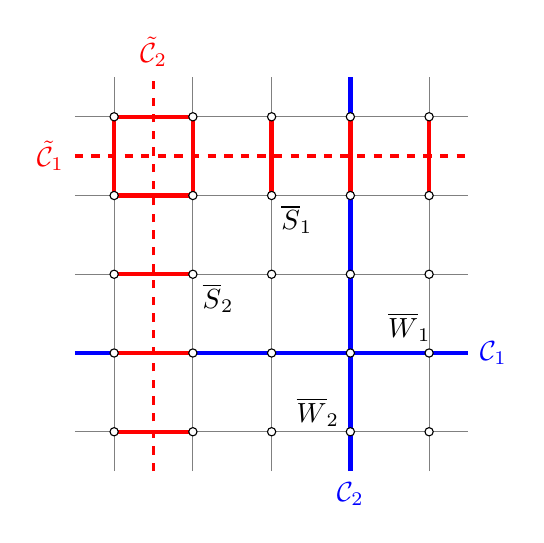
\begin{tikzpicture}[
        site/.style = {circle, inner sep=0 pt, minimum size=3pt, draw=black, fill=white},
    ]
    % lattice grid
    \draw[Gray,thin] (-0.5,-0.5) grid (4.5,4.5);

    % Wilson loops
    \draw[Blue, ultra thick]
        (-0.5, 1) -- (4.5, 1)
        node [pos=1, right] {$\mathcal{C}_1$}
        node [pos=0.85, above, black] {$\overline{W}_1$}
        ;
    \draw[Blue, ultra thick]
        (3, -0.5) -- (3, 4.5)
        node [pos=0, below] {$\mathcal{C}_2$}
        node [pos=0.15, left, black] {$\overline{W}_2$}
        ;

    % 't Hooft strings
    \draw[Red, very thick, dashed]
        (-0.5,3.5) -- (4.5,3.5)
        node[pos=0, left] {$\tilde{\mathcal{C}}_1$}
        ;
    \foreach \x in {0,...,4} { \draw[Red, ultra thick] (\x, 3) -- +(0, 1); }
    \draw (2,3) node [below right] {$\overline{S}_1$};
    \draw[Red, very thick, dashed]
        (0.5,-0.5) -- (0.5,4.5)
        node[pos=1, above] {$\tilde{\mathcal{C}}_2$}
        ;
    \foreach \y in {0,...,4} { \draw[Red, ultra thick] (0, \y) -- +(1, 0); }
    \draw (1,2) node [below right] {$\overline{S}_2$};
    \foreach \y in {0,...,4} \foreach \x in {0,...,4} \draw (\x,\y) node [site] {};
\end{tikzpicture}

    }{Graphical representation of the non-local operators $\Wilson_{1,2}$ (in blue) and $\tHooft_{1,2}$ (in red) and their respective paths $\mathcal{L}_{1,2}$ and $\mathcal{C}_{1,2}$.}
\end{figure}


% These models are akin to the \ac{tc} \cite{kitaev2003fault}, which can be thought as a prime example of a $\Z_2$ \ac{lgt}.
% More precisely, $H_{\Z_2}$ in \eqref{eq:hamiltonian_base} can be thought as a \emph{deformation} of the former, where an external ``transverse'' field is added to it.
% Indeed, using the notation used so far, the \ac{tc} can be formulated as:
% \begin{equation}
%     H_{\text{TC}} = - J_m \sum_{\plaquette} \PlaqOp - J_e \sum_{x} G_x.
%     \label{eq:hamiltoniana_toric_code}
% \end{equation}
% whose ground states $\ket{\Psi}$ satisfies the constraints
% \begin{equation}
%     \PlaqOp \ket{\Psi} = \ket{\Psi} \;\; \forall \; \plaquette, \quad
%     G_x \ket{\Psi} = \ket{\Psi} \;\; \forall x.
%     \label{eq:constraints_gs_toric_code}
% \end{equation}
% Only elementary excitations above the ground state can violate these constraints and they can be of two type: a \emph{magnetic vortex} (which violates the plaquette constraint) or a \emph{electric charge} (which violates the Gauss law).
% If one imposes $J_e \gg J_m$ to enforce Gauss law, in the low-energy sector there are no electric charges and one recovers the pure gauge $\Z_2$ model of \eqref{eq:hamiltonian_base} for $\lambda = 0$.
% Therefore, in general the $\Z_N$ models described in \eqref{eq:hamiltonian_base} can be considered as generalization of the \ac{tc}, from the point of view of \ac{lgt}s.


%
% SUBSECTION: Physical Hilbert space and super-selection sectors
%
\subsection{Physical Hilbert space and super-selection sectors}
\label{sub:physical_hilbert_space_and_super_selection_sectors}


% \todo{Sottosezione da riscrivere in luce della sezione sul toric code}
The total Hilbert space $\mathcal{H}_{\text{tot}}$ is given by
\begin{equation}
    \HilbertSpace_{\text{tot}} = \bigotimes_{\link \in \Lattice} \HilbertSpace_{\link},
\end{equation}
where $\HilbertSpace_\link \simeq \C^N$ in the case of $\Z_N$ theory.
A state of the whole lattice $\ket{\phi_{\phys}} \in \HilbertSpace_{\text{tot}}$ is said to be \emph{physical} if it is a \emph{gauge-invariant state}:
\begin{equation}
    % G_x \ket{\Psi_{\text{ph}}} = \ket{\Psi_{\text{ph}}}, \qquad \forall x \in \lattice
    G_x \ket{\phi_{\phys}} = \ket{\phi_\phys}, \qquad \forall \, x \in \Lattice.
    \label{eq:gauss_law}
\end{equation}
This condition can be translated into a constraint on the eigenvalues $v_{\link}$ of the electric operators $V_{\link}$.
Given that a link $\link$ can be referred to as $(x, \hat{i})$,  then the constraint \eqref{eq:gauss_law} can be translated to
% $v_{(x, \pm \hat{i})}= \omega^{k_{(x, \pm \hat{i})} }$  of the operators $V_\link$ on the links $\link = (x, \pm \hat{i})$ of the vertex $x$:
\begin{equation}
    v_{(x, \hat{1})}^{\phantom{\ast}}
    v_{(x, \hat{2})}^{\phantom{\ast}}
    v_{(x, -\hat{1})}^\ast
    v_{(x, -\hat{2})}^\ast = 1.
\end{equation}
For a $\Z_N$ theory we have $v_\link = \omega^{k_{\link}}$, where $\omega = e^{i2 \pi / N}$, which leads to
% or, because of (\ref{eq:elect_basis_op_action}):
\begin{equation}
    \sum_{i=1,2} \pqty{ k_{(x, \hat{i})} - k_{(x, -\hat{i})} } = 0 \quad \text{mod $N$}.
    \label{eq:gauss_law_elec_eigvals}
\end{equation}
for \eqref{eq:gauss_law}.
Given the fact that the $k$ in \eqref{eq:schwinger_weyl_algebra} represent the values of the electric field, one can see that \eqref{eq:gauss_law_elec_eigvals} can be interpreted as a discretized version of the Gauss law $\nabla \cdot \vec{E} = 0$ in two dimensions, for a pure gauge theory.

% Let us consider the \ac{tc}.
% One of its main features is the presence of topologically protected degenerate ground states \cite{kitaev2003fault}.
Consider now the \emph{physical Hilbert space} for a $\Z_N$ theory:
\begin{equation}
    \Hphys = \{ \ket{\phi_\phys} : G_x \ket{\phi_\phys} = \ket{\phi_\phys} \quad \forall \, x \in \Lattice \}.
    \label{eq:decomposizione_Hphys}
\end{equation}
This space can be decomposed into super-selection sectors, like it has been done for the $\Z_2$ theory in Sec.~\ref{sub:super_selection_sectors}.
In fact, it can be generalized in a straightforward way, using the string operators in \eqref{eq:nonlocal_op_ZN} (showed in Fig.~\ref{fig:nonlocal_operators}).
The physical Hilbert space $\Hphys$ decomposes as
\begin{equation}
    \Hphys = \bigoplus_{n,m=0}^{N-1} \Hphys^{(n,m)},
\end{equation}
where each sector $(n,m)$ satisfy
\begin{equation}
    S_1 \ket{\phi} = \omega^{m} \ket{\phi}
    \qand
    S_2 \ket{\phi} = \omega^{n} \ket{\phi}
\end{equation}
for $\ket{\phi} \in \Hphys^{(n,m)}$.
This is possible because the \ac{ths}s $\tHooft$ commutes with all the terms of the Hamiltonian.

On the other hand, the $\Wilson_i$ do not commute with all the terms in the Hamiltonian \eqref{eq:hamiltonian_base}, in particular with the electric operators $V_{\link}$, but are still gauge-invariant.
Nonetheless, we are interested in the commutation relation between the \ac{wl}s and \ac{ths}s:
\begin{equation}
    \Wilson_1 \tHooft_2 = \omega \tHooft_2 \Wilson_1
    \qand
    \Wilson_2 \tHooft_1 = \omega \tHooft_1 \Wilson_2.
    \label{eq:relation_W_S_ZN}
\end{equation}
It is a direct generalization of the relations \eqref{eq:anticommutation_W_S_toric} of the \ac{tc}, where the sign $-1$ is upgraded to a characteristic phase $\omega$.
Given \eqref{eq:relation_W_S_ZN}, it is easy to see that the \ac{wl}s have the ability to change the super-selection sectors:
\begin{equation}
    W_1 : \Hphys^{(n,m)} \to \Hphys^{(n+1,m)}
    \qand
    W_2 : \Hphys^{(n,m)} \to \Hphys^{(n,m+1)},
    \label{eq:azione_wilson_loop}
\end{equation}
where the addition is taken modulus $N$.

From a physical point of view, the \ac{wl}s operators create non-contractible electric loops around the lattice, while the \ac{ths}s detect the presence and the strength of these electric loops, by traversing it in the orthogonal direction.
Exactly like in the case of the $\Z_2$ \ac{lgt}, but the difference that now the non-contractible electric strings can have different ``strengths'', given by the different eigenvalues of $\tHooft_i$.
Therefore, it is clear that the Hilbert subspace $\Hphys^{(n, m)}$ is the subspace of all the states that contains an electric loop of strength $\omega^n$ and $\omega^{m}$ along the $\hat{1}$ and $\hat{2}$ direction, respectively.

Furthermore, the evolution of a state in $\Hphys^{(n,m)}$ with the Hamiltonian in \eqref{eq:hamiltonian_base} is confined in $\Hphys^{(n,m)}$.
This is because none of the local terms in the Hamiltonian can change the super-selection sector, only the non-local \ac{wl}s.
In this chapter we will see how this fact can have major consequences when considering $\Z_N$ models on particular lattice geometries, in particular on the \emph{ladder}.
